\section{Clustering par partionement}
Nous avons réalisé le clustering par partitionnement à l'aide du composant hierarchical Clustering avec la configuration Linkage type : COMPLETE. Pour observer les résultats nous avons utilisé le composant Scatter Matrix.

\paragraph{Santé}
Nous avions choisi de faire 3 clusters (cf section précédente), voici les résultats obtenus : 

\begin{figure}[H]
	\begin{center}
		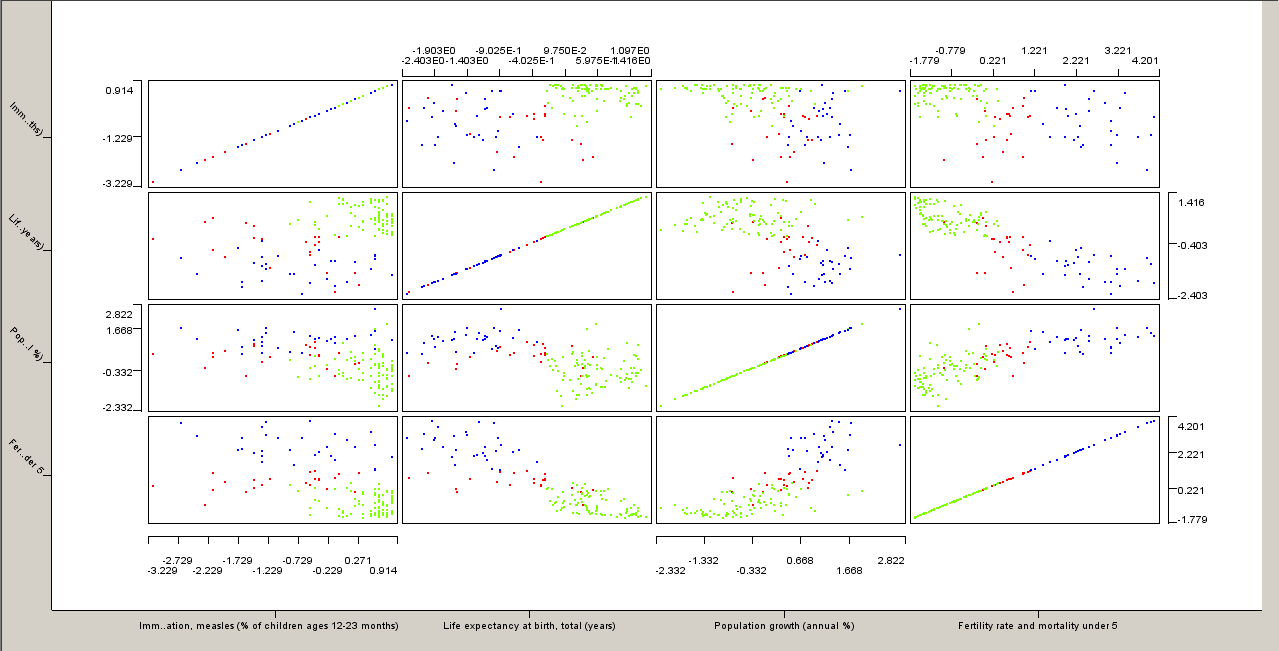
\includegraphics[scale=0.5]{Image/ScatterMatrixSanteNoMissing2}
		\caption{Scatter Matrix des attributs de l'indicateur Santé \jeuc}
	\end{center}
\end{figure}

